%!TEX root = ../dokumentation.tex

\chapter{Theoretische Grundlagen}
\section{Maxwellsche Gleichungen}
Das Fundament des Elektromagnetismus lässt sich in partiellen Differentialgleichungen zusammenfassen. Dieses Gleichungssystem wird häufig auch als die \" Maxwellsche Gleichungen \" bezeichnet:
\[div \vec{D} = \rho\]
\[rot \vec{E} = -\div{}\]
%TODO
\section{Elektromagnetische Wellen}
Als elektromagnetische Welle werden räumlich ausbreitende Wellen bezeichnet, die aus elektrischen und magnetischen Feldern besteht. Die laufende Welle breitet sich entlang der Ausbreitungsgeschwindigkeit mit einer Geschwindigkeit von \[c= 3*10^8 m/s\] aus. Die elektrischen und magnetischen Feldvektoren der Welle stehen orthogonal aufeinander, wie in der Abbildung \ref{elektromagnetische Welle} gut zu erkennen.

\begin{figure}[ht]
	\centering
	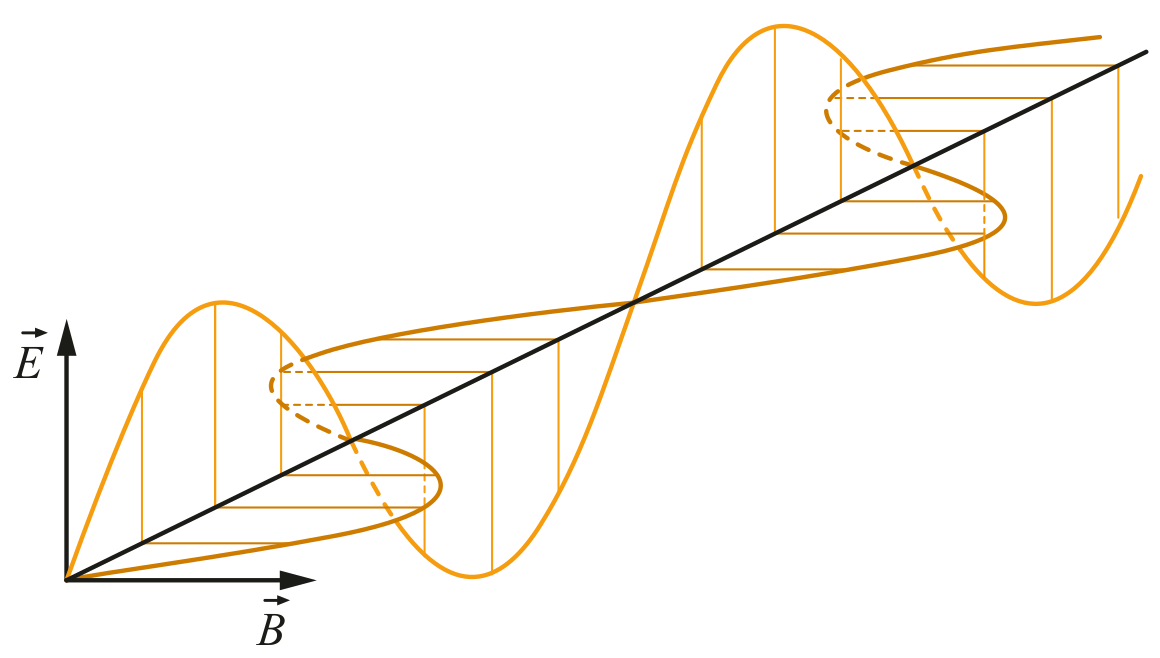
\includegraphics[width=0.75\textwidth]{em-welle.png}
	\caption[Elektromagnetische Welle mit senkrecht
	aufeinander stehendem elektrischem und magnetischem Feld]{Elektromagnetische Welle mit senkrecht aufeinander stehendem elektrischem und magnetischem Feld. Quelle: \cite[Harten, S. 130]{Harten:2017}} 
	\label{elektromagnetische Welle}
\end{figure}

Der Frequenzbereich, auch Spektrum einer solchen elektromagnetischen Welle reicht von langsamen Radiowellen, Infrarotwellen über den Bereich des sichtbaren Lichts bis hin zur Röntgenstrahlung und der extrem kurzwelligen Gammastrahlung. In der Abbildung \ref{frequenzbereiche} werden die Frequenzbereiche detaillierter dargestellt.

Die elektromagnetischen Wellen, die auf unsere Erde einwirken werden auch natürliche Strahlung genannt. Sie ermöglicht das Leben auf der Erde, da die Energiezufuhr des Lebens auf der Erde über infrarot Wellen der Sonne gegeben ist.
Elektromagnetische Wellen benötigen kein Medium, um sich auszubreiten. Sie können sich daher auch über weiteste Entfernungen ausbreiten. Sie bewegen sich im Vakuum unabhängig von ihrer Frequenz mit Lichtgeschwindigkeit fort. Elektromagnetische Wellen können sich aber auch in Materie ausbreiten wie etwa Gas oder Flüssigkeit, jedoch verringert sich dabei ihre Geschwindigkeit.

Die Existenz der elektromagnetischen Wellen folgt aus den Maxwell-Gleichungen. Sie wurden 1886 von H.Hertz erstmals durch den elektrischen Schwingkreis erzeugt.

\subsection{Eigenschaften einer elektromagnetischen Welle}
%TODO
\subsection{Elektronisches Rauschen}
Rauschen im Allgemeinen ist der Oberbegriff für Störspannungen, die ein Nutzsignal überlagern. Es wird als unerwünschtes Signal bezeichnet, das in Kommunikationssystem leider allgegenwärtig ist. Das Rauschen behindert den Empfang von Nachrichten bei der Übertragung, deshalb ist es erforderlich diesen Nebeneffekt zu begrenzen. Rauschen kann mehrere Ursachen haben, die alle durch physikalische Gesetzmäßigkeiten begründet werden können. Üblicherweise sind  Rauschen zufällig auftretende Störspannungen, die keine  Phasen oder Frequenzbeziehung zueinander haben.
%TODO

\newpage
\section{Nachrichten- und Übertragungstechnik}
Die Nachrichten- und Übertragungstechnik beschäftigt sich mit dem Übertragen elektronischer Nachrichten. Als Nachricht wird in diesem Kontext ein vom Sender gezielt erzeugtes Signal verstanden, welches mit Informationen behaftet und für den Empfänger der Nachricht bestimmt ist \cite[vgl. Werner, S. 3]{Werner:2006}.

Das in Abb. \ref{nachrichtenuebertragung} dargestellte Kommunikationsmodell nach Shannon beschreibt den Grundlegenden Aufbau eines Nachrichtenaustausches zweier Systeme. 
Im Folgenden werden die zum weiteren Verständnis notwendigen Begriffe eingeführt:\newline
Die Informationsquelle (\enquote{Information Source}) übergibt die Nachricht dem Sender (\enquote{Transmitter}), der diese mit einem Signal als physikalischem Träger der Nachricht über einen Kanal (\enquote{Channel}) sendet. \newline
Als Kanal bezeichnet man in der Nachrichtentechnik sämtliche technische Komponenten, welche eine Information vom Sender zum Empfänger transportiert. \cite[vgl. Dankmeier, S. 13]{Dankmeier:2017}.\newline
Die im Kanal auftretenden Störsignale, hier durch die Störsignalquelle (\enquote{Noise Source}) dargestellt, überlagern sich mit dem ursprünglichen Signal. Aus dem für den Empfänger (\enquote{Receiver}) bestimmten Empfangssignal (\enquote{Received Signal}) wird anschließend wieder eine Nachricht generiert, die im letzten Schritt der Informationssenke (\enquote{Destination}) übergeben wird.

\begin{figure}[ht]
	\centering
	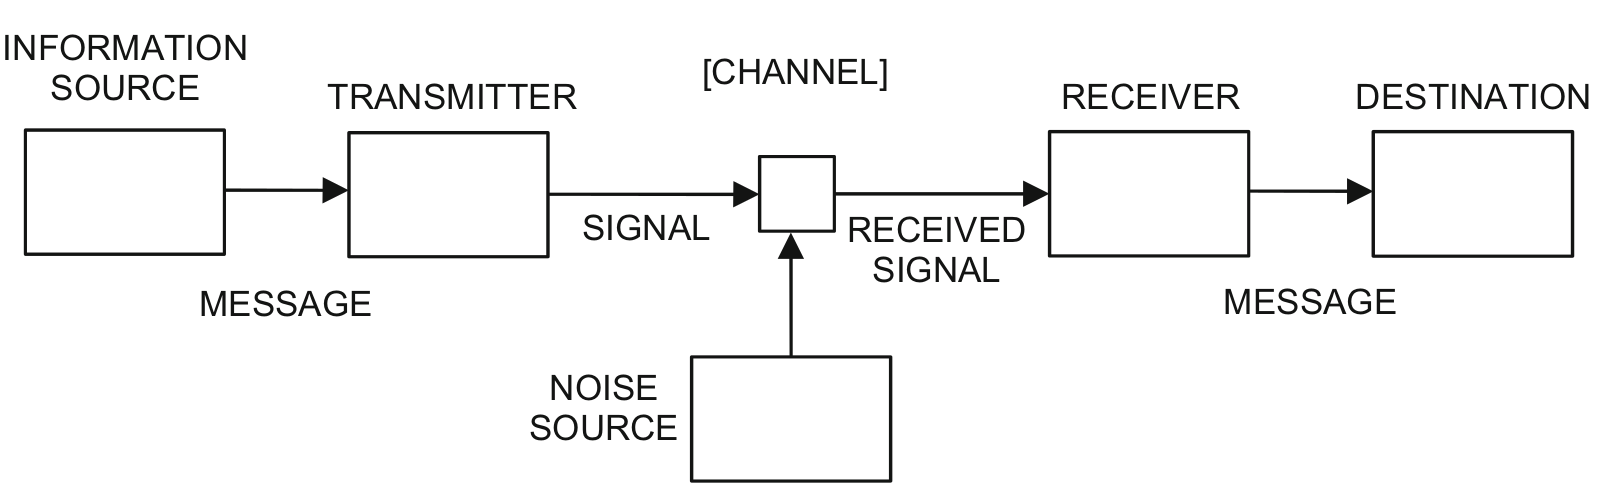
\includegraphics[width=\textwidth]{nachrichtenuebertragung-shannon.png}
	\caption[Kommunikationsmodell nach Shannon]{Kommunikationsmodell nach Shannon. Quelle: \cite[Werner, S. 11f]{Werner:2017}} 
	\label{nachrichtenuebertragung}
\end{figure}

\section{Signale und Spektren}
Signale werden üblicherweise auf 2 Arten dargestellt:
\begin{enumerate}
	\item Als \textit{Signal} im Zeitbereich
	\item Als \textit{Spektrum} im Frequenzbereich
\end{enumerate}

\subsection{Kontinuierliche und diskrete Signale}
Als Signal gilt eine Funktion mit mindestens einer unabhängigen Variablen, beispielsweise der Zeit \(t\). Ist die Zeitvariable nur für diskrete Werte definiert, so spricht man von einem zeitdiskreten Signal. Man schreibt auch \(x[n]\), wobei \(n\) die normierte Laufvariable genannt wird \cite[vgl. Werner, S. 24]{Werner:2017}.

In Abb. \ref{kontinuierlich_diskret} wird das kontinuierliche Signal
\[x(t) = \sin \omega t = \sin 2\pi f t\]
mit \(f = 50 \text{ Hz} \) dargestellt und mit dem diskreten Signal
\[x[n] = x(nT_a) = \sin 2\pi f T_a n\]
überlagert, welches mit einer Abtastrate von \(f_a = 1 \text{ kHz}\) oder anders ausgedrückt: einem Abtastintervall von \(T_a = 1 / f_a = 1 \text{ ms}\) abgetastet wird \cite[vgl. Heuberger, e. a., S. 11f]{Heuberger:2017}.

\begin{figure}[ht]
	\centering
	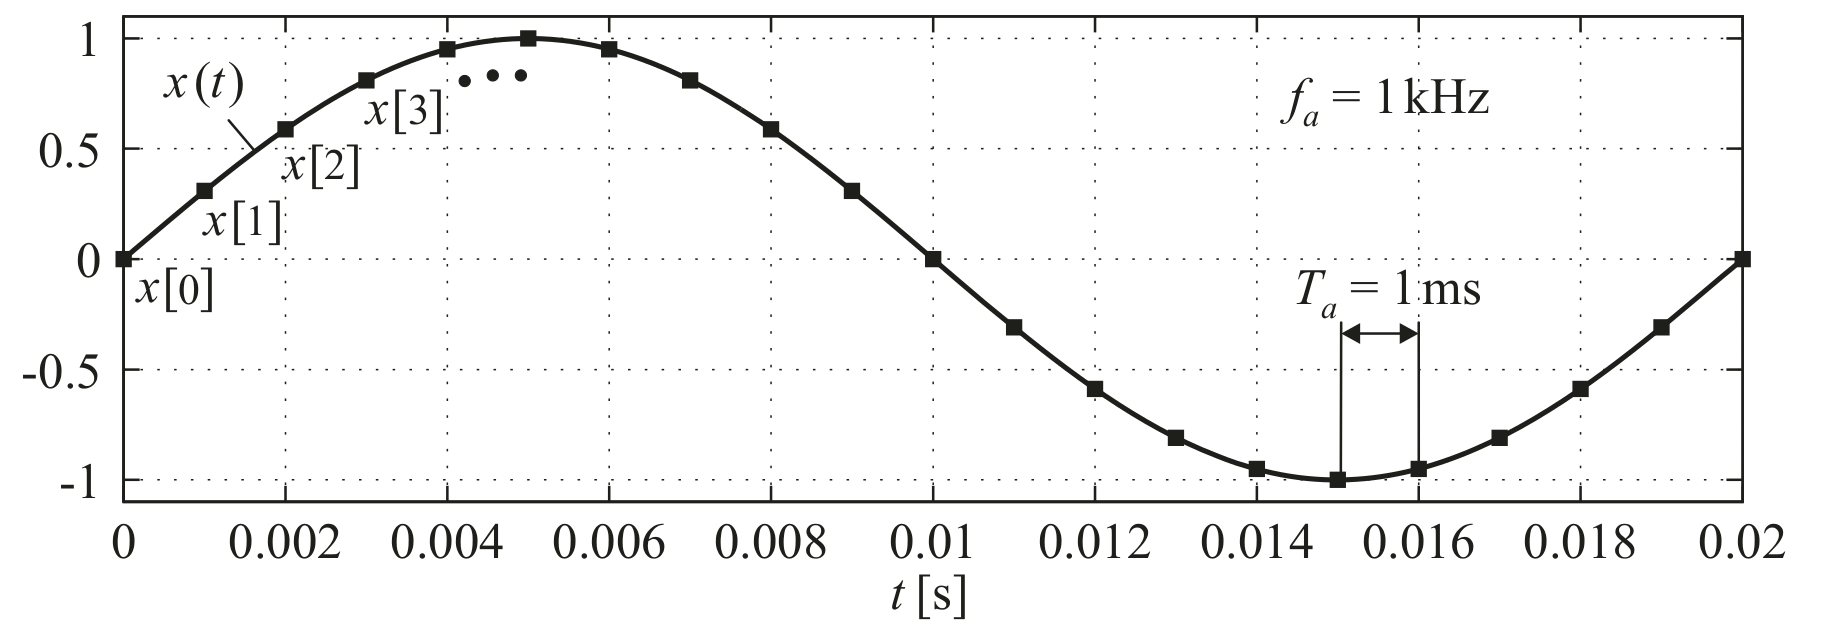
\includegraphics[width=\textwidth]{kontinuierlich-diskret.png}
	\caption[Sinus-Signal als kontinuierliches und als diskretes Signal]{Sinus-Signal als kontinuierliches und als diskretes Signal. \newline Quelle: \cite[Heuberger, e. a., S. 12]{Heuberger:2017}} 
	\label{kontinuierlich_diskret}
\end{figure}
%\subsection{Analoge und digitale Signale}
%Digitale Signale sind sowohl werte- als auch zeitdiskret.

\subsection{Spektrum eines Signals}
Eine alternative Darstellung von Signalen kann im Frequenzbereich erfolgen. Dort wir ein Signal mit einzelnen Sinus-Schwingungen beschrieben, aus denen es sich zusammensetzen lässt \cite[vgl. Karrenberg, S. 42]{Karrenberg:2017}.

\subsubsection{Fourier-Transformation}
Um ein Signal aus dem Zeitbereich in den Frequenzbereich zu überführen wird die sogenannte Fourier-Transformation verwendet.\newline
Im wesentlichen wird ein Signal bzw. eine Funktion mittels Fourier-Transformation als Summe mehrerer Sinus-Schwingungen unterschiedlicher Frequenzen und Amplituden dargestellt.

Signale können also entweder aus Sinusschwingungen konstruiert, oder in solche zerlegt werden.
Nach der Zerlegung ergeben sich einige Möglichkeiten mit den einzelnen Frequenzen zu arbeiten:
\begin{itemize}
	\item Aus einem Signal können einzelne Frequenzen hervorgehoben werden
	\item Bei Audiosignalen beispielsweise können ungewollte Frequenzen ausgeblendet werden (etwa Hintergrundrauschen)
\end{itemize}

Um von dem resultierenden Spektrum wieder zu einer Darstellung im Zeitbereich zu gelangen, kann die Umkehroperation, die inverse Fourier-Transformation angewandt werden.

In der Praxis wird für die Überführung in den Frequenzbereich meist die \ac{FFT} genutzt \cite[vgl. Heuberger, e. a., S. 14]{Heuberger:2017}.

Um ein Signal mittels \ac{FFT} in den Frequenzraum überführen zu können, muss es die Länge der Form \(N = 2^L\) aufweisen. \(N\) muss also eine 2er-Potenz sein \cite[vgl. Heuberger, e. a., S. 15]{Heuberger:2017}.
Für das zu überführende Signal gilt also:
\[\underline{x} = \Big[ \:  \underline{x}[0] \; \underline{x}[1] \; \underline{x}[2] \; ... \; \underline{x}[N - 2] \; \underline{x}[N - 1] \; \Big] \]

\subsubsection{Fensterfunktionen}
In der Praxis, so auch bei \ac{SDR}-Systemen, handelt es sich in der Regel um Ausschnitte eines Signales. Bei der \ac{FFT} wird mit periodischen Signalen gearbeitet, ein Signalausschnitt ist aber nur quasiperiodisch. Denn an den Rändern gibt es bei der periodischen Fortsetzung des Signals Sprungstellen \cite[vgl. Meyer, S. 187]{Meyer:2017}.\newline
Wird also ein Signal, dessen Länge kein vielfaches einer ganzen Periode ist, aufgezeichnet, entsteht durch die Unstetigkeiten am Rand eine spektrale Streuung durch die Umwandlung mit der \ac{FFT}.

Der Signalausschnitt wird deshalb mit einer sogenannten Fensterfunktion gewichtet: 
\[w = \Big[ \:  w[0] \; w[1] \; w[2] \; ... \; w[N - 2] \; w[N - 1] \; \Big] \]


Die gefensterte FFT Funktion:
\[\text{FFT} _w \: {\underline{x}[n]} = \sum_{n=0}^{N-1} w[n] \: \underline{x}[n] \: e^{-j2\pi nm / N} \text{ mit } m = 0, ..., N-1\]


Das Spektrum dieser Funktion lässt sich als den gewichteten Betrag des resultierenden Ergebnisses ausdrücken \cite[vgl. Heuberger, e. a., S. 14]{Heuberger:2017}:
\[s_x[m] = \frac{1}{c_w^2} \: \Big{|}\underline{X}[m]  \Big{|}^2 \text{ mit } c_w = \sum_{n=0}^{N-1} w[n] \]

In Abbildung \ref{fft} wird das diskrete Zeitsignal \(x[n]\) dem gefensterten Zeitsignal \(w[n]x[n]\) und dem aus der FFT resultierenden Spektrum \(S_x[m]\) gegenübergestellt:
\begin{figure}[ht]
	\centering
	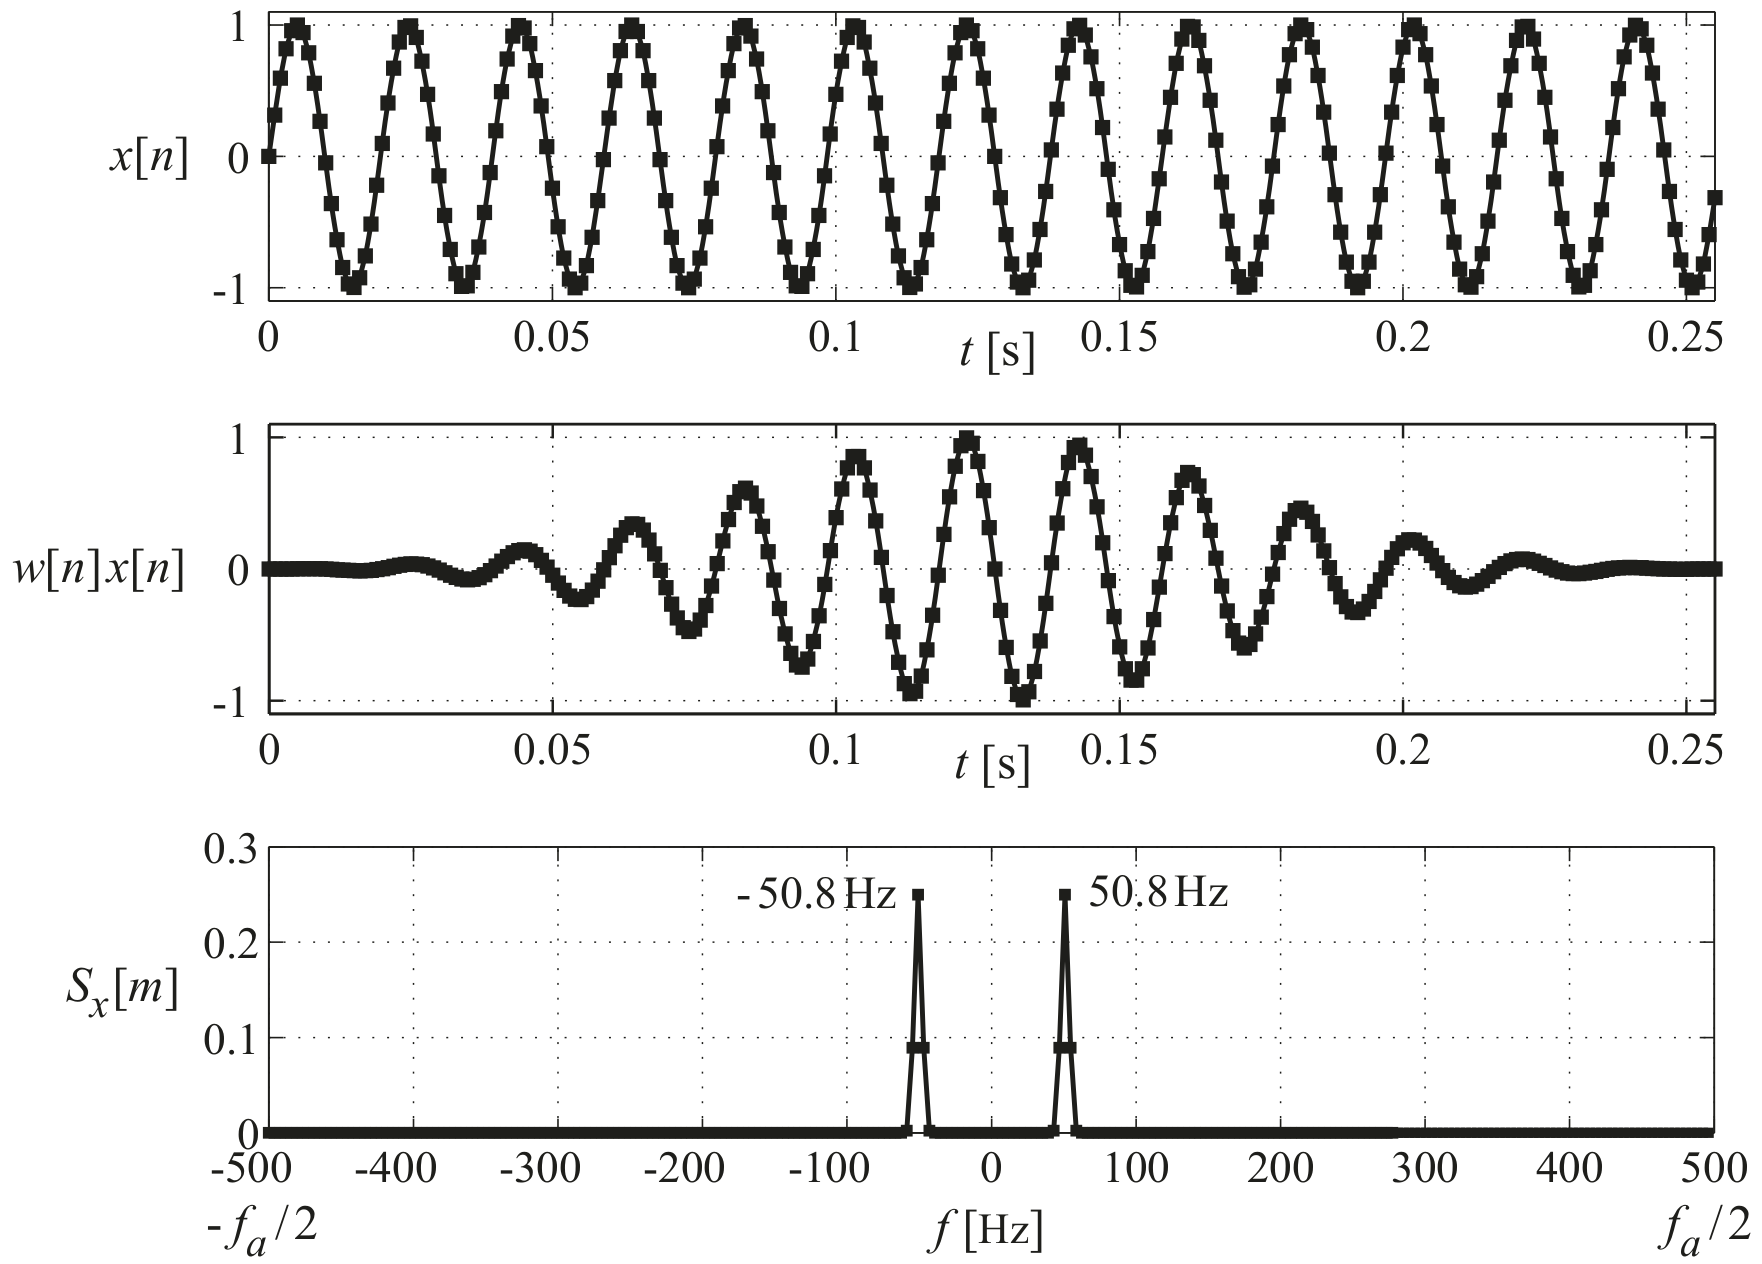
\includegraphics[width=\textwidth]{FFT.png}
	\caption[Zeitsignal, gefenstertes Zeitsignal und Spektrum eines diskreten Sinus-Signals]{Zeitsignal, gefenstertes Zeitsignal und Spektrum eines diskreten Sinus-Signals. Quelle: \cite[Heuberger, e. a., S. 16]{Heuberger:2017}} 
	\label{fft}
\end{figure}

\section{Nyquist-Shannon-Abtasttheorem}

\newpage
\section{Frequenzbereiche}
Zur Orientierung im Spektrum elektromagnetischer Wellen haben sich international verschiedene Systeme zur Klassifikation sogenannter Frequenzbänder gebildet. Die \ac{ITU} empfiehlt eine Einteilung des Spektrums von 3 kHz bis 300 GHz in acht Frequenzbereiche, auch Frequenzdekaden genannt. \cite[vgl. ITU-R v.431-8]{itu-431:2015}

\begin{figure}[ht]
	\centering
	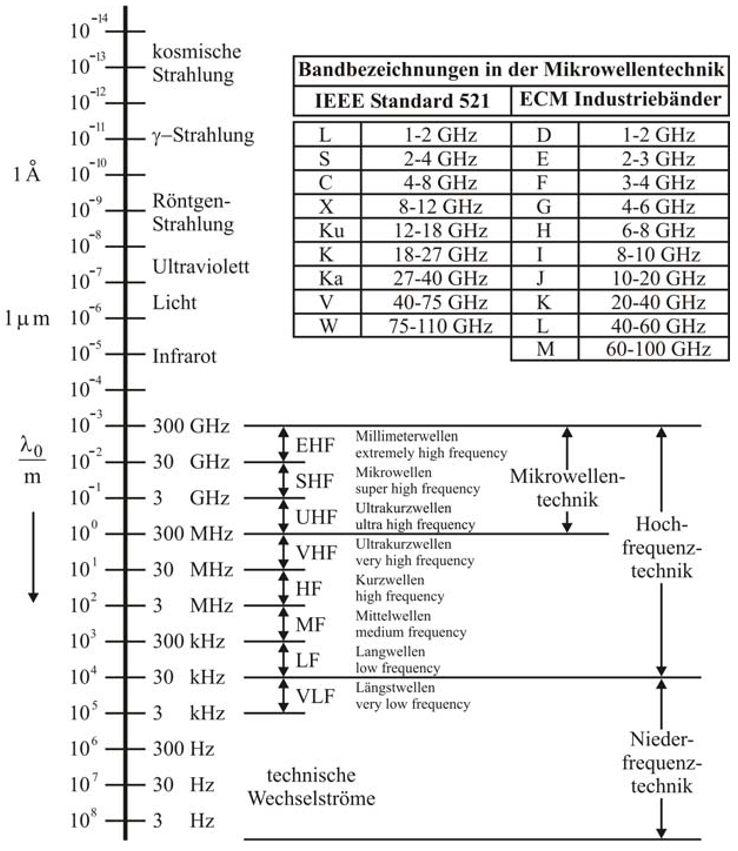
\includegraphics[width=0.75\textwidth]{frequenzbereich.png}
	\caption[Spektrum elektromagnetischer Wellen und gebräuchliche Bandbezeichnungen]{Spektrum elektromagnetischer Wellen und gebräuchliche Bandbezeichnungen. Quelle: \cite[Kark, S. 1]{Kark:2017}} 
	\label{frequenzbereiche}
\end{figure}


\subsection{Rechtliche Grundlagen} %TODO
In Deutschland gilt rechtlich zudem die Aufteilung des Frequenzbereiches von 9 kHz bis 3000 GHz, welche von der Bundesnetzagentur im sogenannten Frequenzplan \cite[Bundesnetzagentur, 2016]{bundesnetzagentur-frequenzplan:2016} gemäß § 54 TKG festgehalten wird.
Dort werden die Frequenzbereiche nach Frequenznutzung (Amateurfunk, Seefunk, WLAN, etc.) eingeteilt und entsprechende Nutzungsbestimmungen spezifiziert:

\begin{figure}[ht]
	\centering
	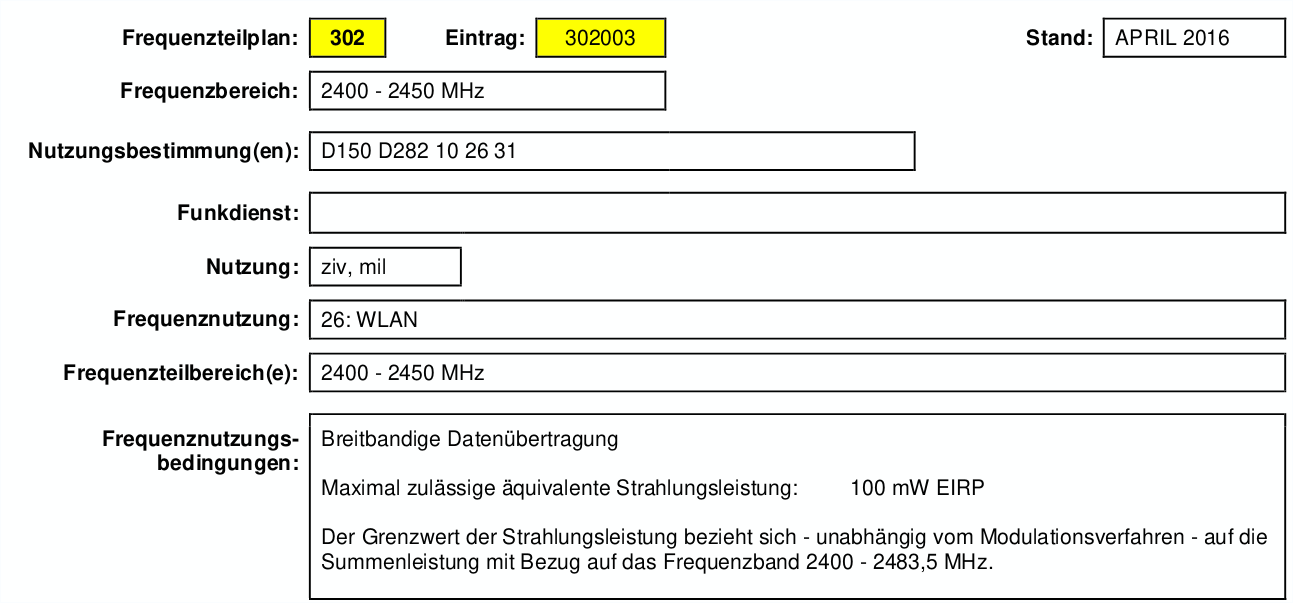
\includegraphics[width=\textwidth]{freqplan-wlan.png}
	\caption[Eintrag: 2,4 GHz WLAN im Frequenzplan]{Eintrag: 2,4 GHz WLAN im Frequenzplan. Quelle: \cite[Bundesnetzagentur, 2016]{bundesnetzagentur-frequenzplan:2016}}
	\label{frequenzplan-wlan}
\end{figure}

\subsection{Dezimeterwelle}
Das Frequenzband von 300 MHz bis 3 GHz, auch \ac{UHF}-Band genannt, ist ein Frequenzbereich in dem die Wellen eine Länge von zehn Dezimeter bis einem Dezimeter besitzen.

\section{Bluetooth}
Bluetooth ist eine Übertragungstechnik für kabellose Kommunikation über kurze Distanzen. Es wird im Frequenzbereich von 2,4 bis 2,4835 GHz betrieben \cite[Bundesamt für Strahlenschutz, S. 1]{bundesamt-strahlungsschutz:2012}. Insgesamt gibt es unter Bluetoothgeräten drei verschiedene Sendeleistungsklassen:
\begin{description}
	\item[Klasse 1: bis 1,0 mW] Reichweite: bis 10m 
	\item [Klasse 2: bis 2,5 mW] Reichweite: 10m und mehr
	\item [Klasse 3: bis 100 mW] Reichweite: 100m und mehr
\end{description}
Die Aufteilung des Frequenzbereiches von 0 kHz bis 3000 GHz wird von der Bundesnetzagentur im sogenannten Frequenzplan \cite[Bundesnetzagentur]{bundesnetzagentur-frequenzplan:2016} gemäß § 54 TKG festgehalten.

\section{Wireless Local Area Network}
Unter dem Begriff Wireless Local Network (WLAN) versteht man ein kabelloses lokales Netzwerk, welches meist an Orten eingesetzt wird, bei der kabelgebundene Datenübertraung zu teuer, umständlich oder umkomfortabel wäre.

\section{Software Defined Radio} 
\enquote{Funkübertragungssysteme, bei denen wesentliche Teile der Verarbeitung mittels Software erfolgen, werden als Software Defined Radio \ac{SDR}-Systeme bezeichnet.} \cite[Heuberger, e. a., S. 1]{Heuberger:2017}


